%%% Local Variables:
%%% mode: latex
%%% TeX-master: "../doc"
%%% coding: utf-8
%%% End:
% !TEX TS-program = pdflatexmk
% !TEX encoding = UTF-8 Unicode
% !TEX root = ../doc.tex

\section{Survey Instrument (UniPark Export)}
\label{appendix:survey}
% First page with title on same page
\begin{center}
  \centering
  \makebox[\textwidth][c]{%

    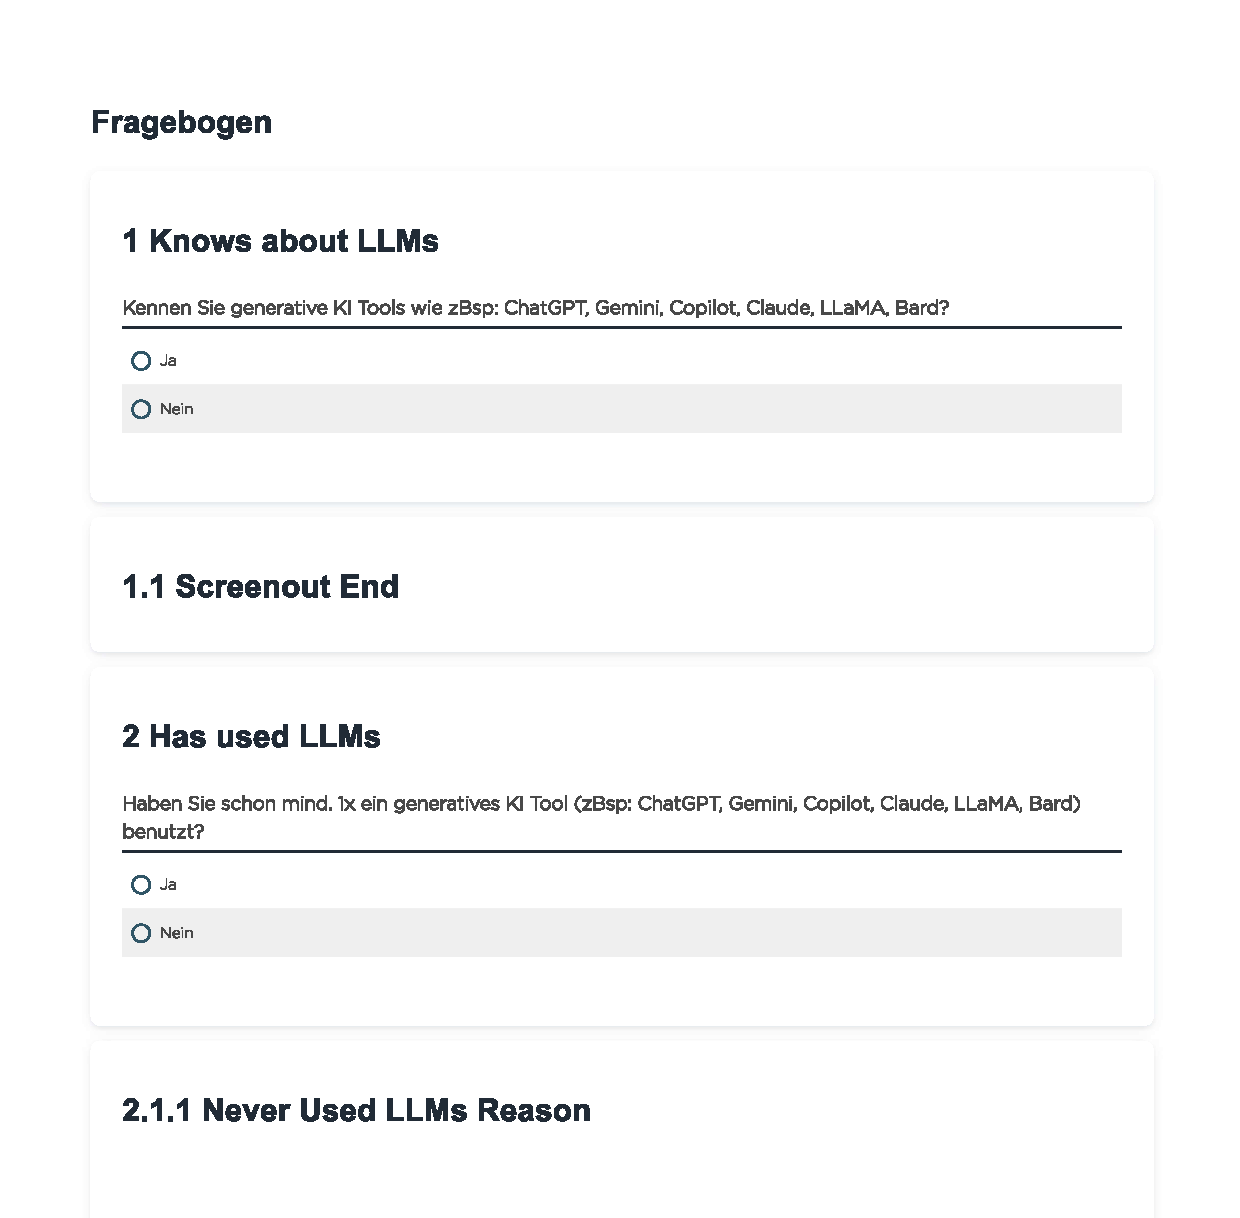
\includegraphics[page=1,width=1.3\textwidth]    {resources/full_questionnaire_cropped.pdf}
    }
\end{center}
%TODO: uncomment for final render
\includepdf[pages={2-30,32-},scale=0.99]{resources/full_questionnaire_cropped}

\section{Additional Survey Results}
\label{appendix:survey_result_addons}
\begin{figure}[htbp]
    \centering
  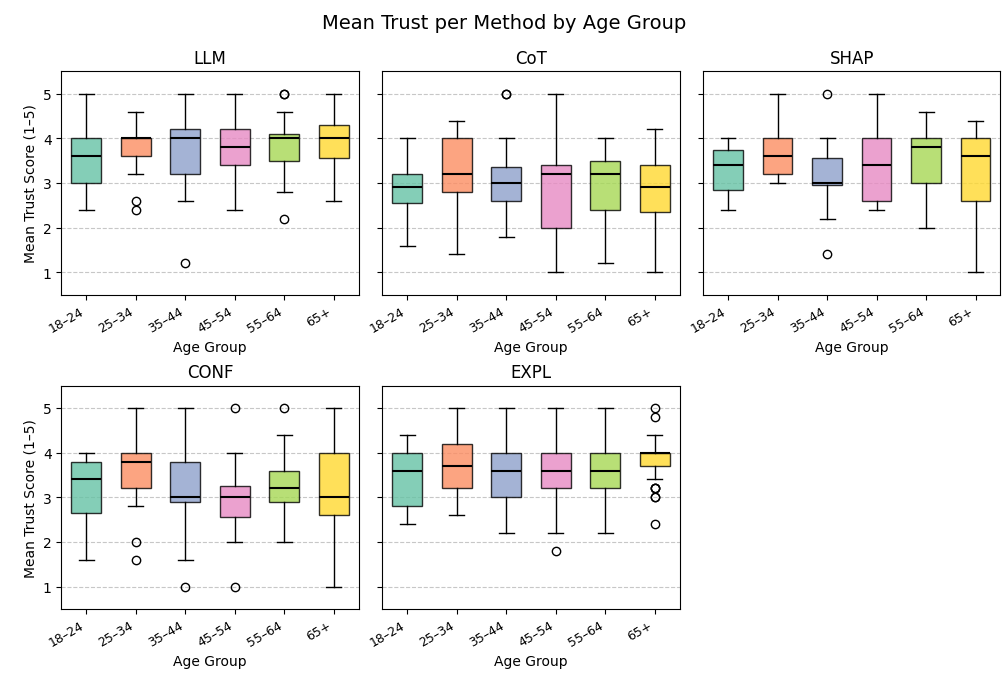
\includegraphics[width=1\textwidth]{diagrams/survey_diagrams/age_trust_boxplot.png}
  
    \caption{Mean Trust per Method by Age Group}
\end{figure}

\begin{figure}[htbp]
  \centering
  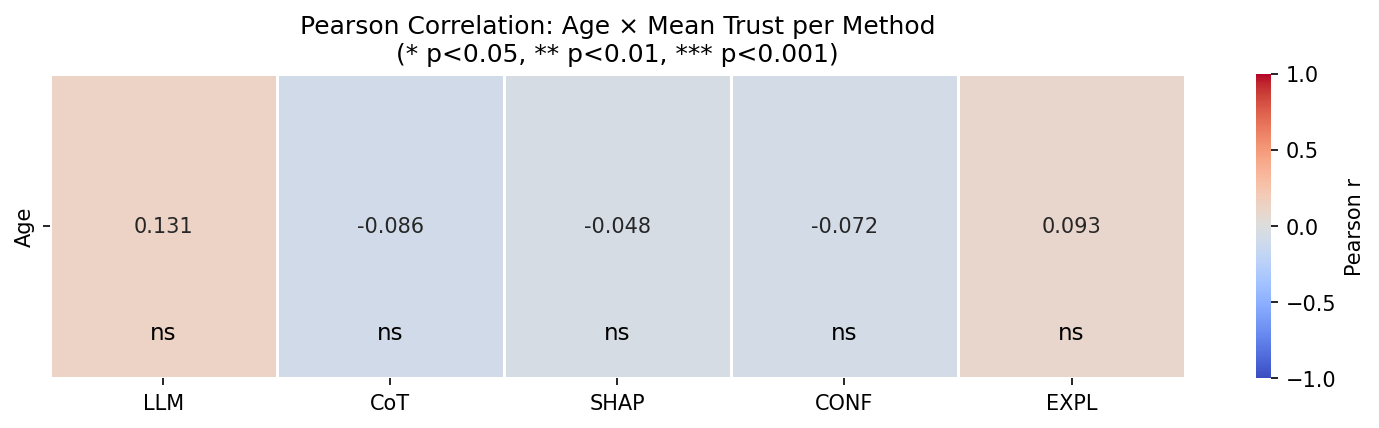
\includegraphics[width=0.9\textwidth]{diagrams/survey_diagrams/age_trust_heatmap.png}
  \caption{Pearson Correlation Age x Mean Trust}
\end{figure}

\begin{figure}[htbp]
  \centering
  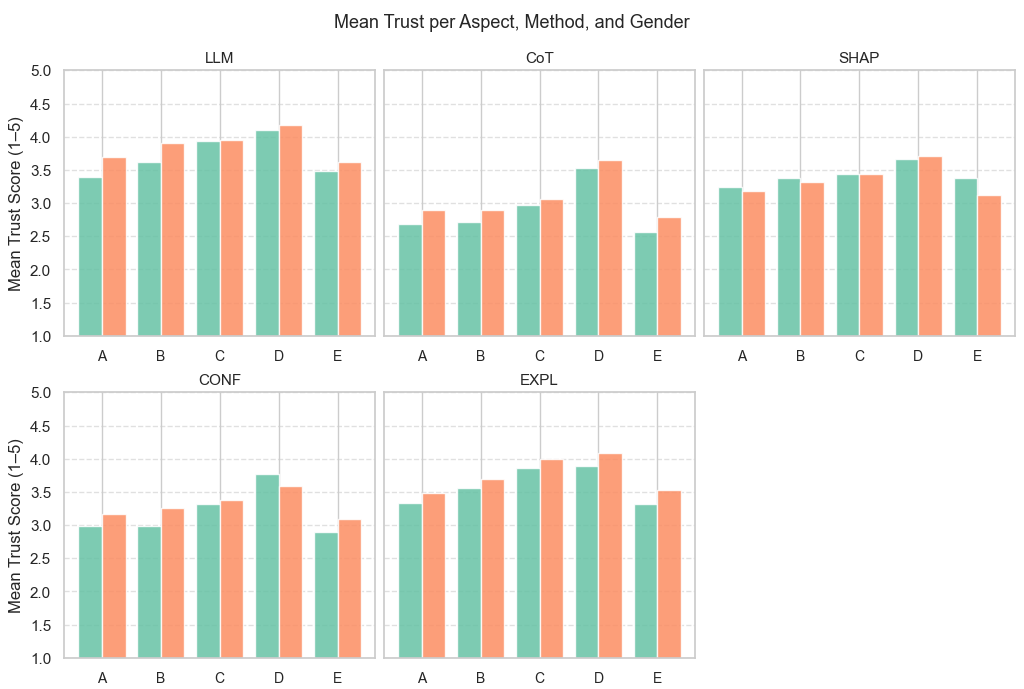
\includegraphics[width=1\textwidth]{diagrams/survey_diagrams/gender_trust_aspect_bars.png}
  
  \caption{Mean Trust per Aspect, Method and Gender\\ A = Factually Accurate, B = Reliable, C = Competent and Knowledgeable, D = Tried to answer correctly, E = Would rely on answers}
\end{figure}

\begin{figure}[htbp]
  \centering
  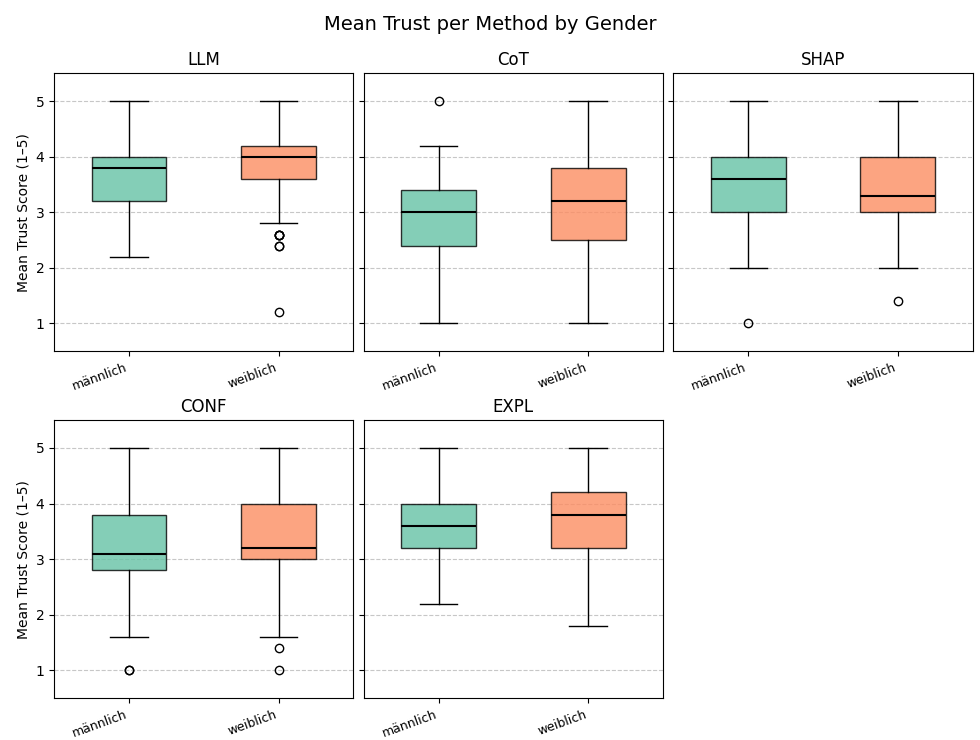
\includegraphics[width=1\textwidth]{diagrams/survey_diagrams/gender_trust_boxplot.png}
  
  \caption{Mean Trust per Method by Gender}
\end{figure}

\begin{figure}[htbp]
  \centering
  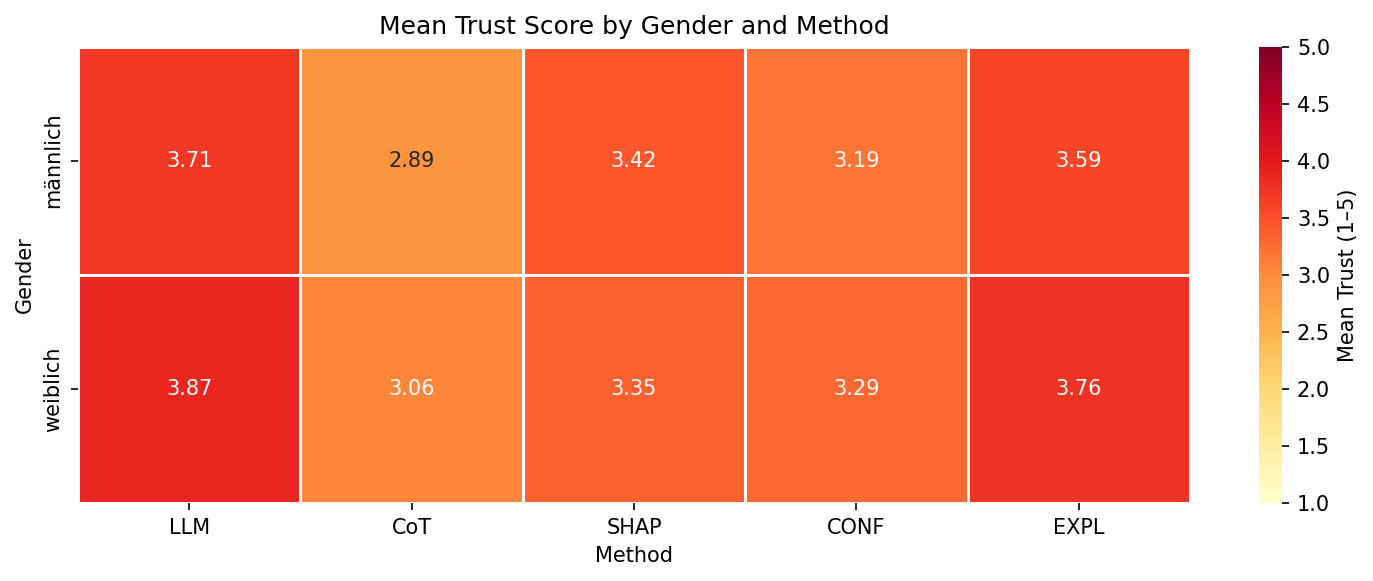
\includegraphics[width=0.7\textwidth]{diagrams/survey_diagrams/gender_trust_heatmap.png}
  \caption{Trust Score by Gender and Method}
\end{figure}

\begin{figure}[htbp]
  \centering
  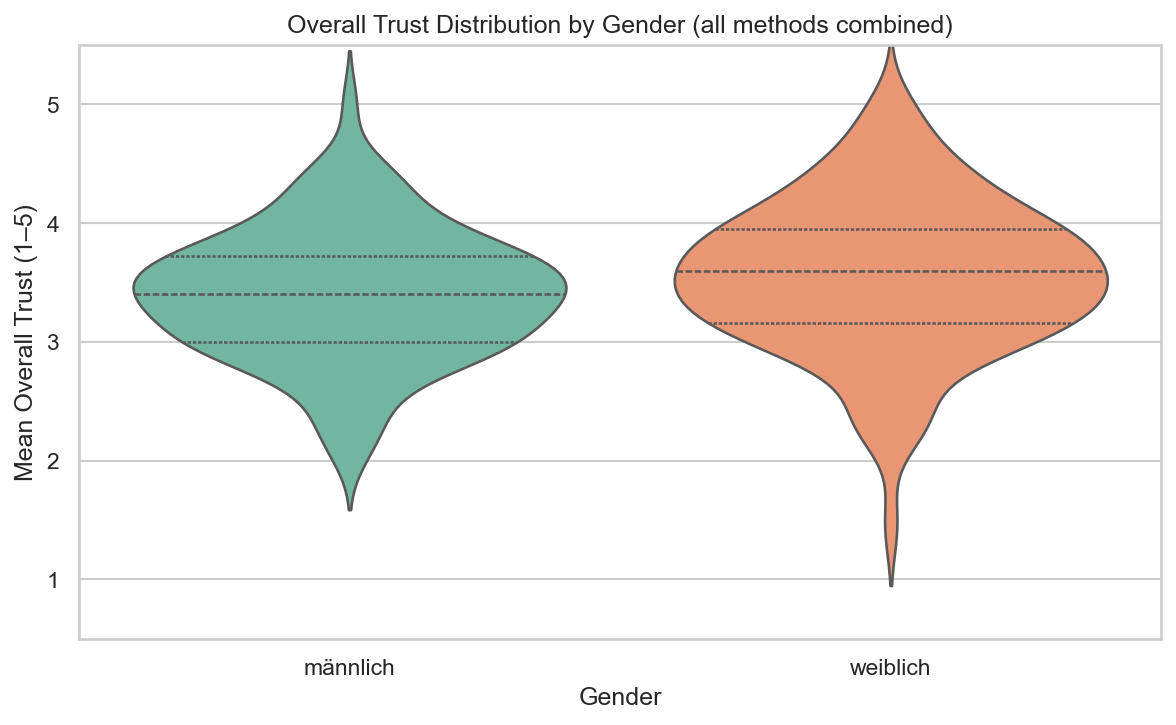
\includegraphics[width=0.8\textwidth]{diagrams/survey_diagrams/gender_trust_violin.png}
  \caption{Trust distribution by Gender}
\end{figure}

\begin{figure}[htbp]
  \centering
  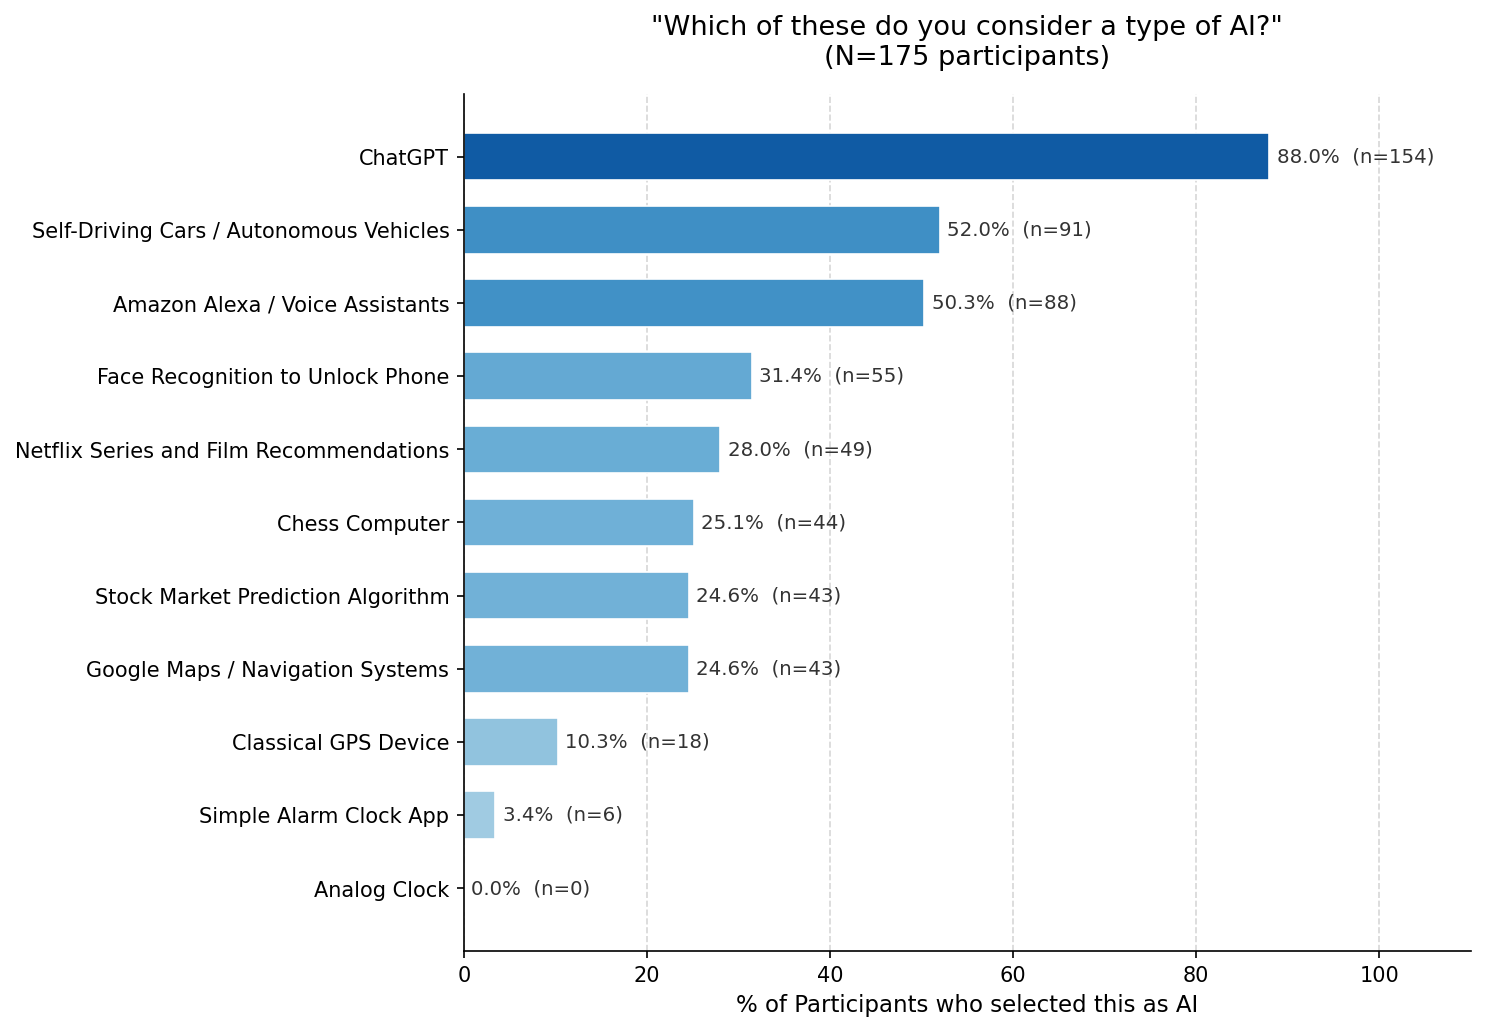
\includegraphics[width=\textwidth]{diagrams/survey_diagrams/typeofai_barplot.png}
  \caption{Applications considered to be AI by Participants}
\end{figure}
